\chapter[Isostasy]{Isostasy\\ \large Gravity Extension}\label{ch:isostasy}

\section*{Introduction}

Isostasy refers to an equilibrium state of buoyancy, much like an iceberg floating in the ocean.  Approximately 10\% of an iceberg rises above the water surface, with the remaining 90\% hidden from view.  For icebergs of different size, larger ice masses extend both higher above and deeper below the waterline.  Placing a series of icebergs side by side would produce relief above the surface and compensating roots below, a configuration that closely parallels topography and its subsurface support within the Earth.

\emph{Isostasy} describes a state of mechanical equilibrium in which \emph{lateral variations} in mass (loads) are arranged such that pressure is balanced at a common depth, known as the \emph{depth of compensation}.  Isostasy is an equilibrium condition, not a physical process.  The mechanisms by which the Earth approaches or departs from this state—such as elastic flexure, viscous mantle flow, erosion, sedimentation, and thermal contraction—are referred to as \emph{isostatic processes}.  Throughout this chapter, we will distinguish carefully between isostasy as a state and isostatic processes as the means by which that state is modified or restored.

Because isostatic balance depends on vertically integrated mass, it carries no intrinsic vertical resolution.  Different distributions of density and thickness can satisfy the same isostatic condition.  Moreover, the presence of lithospheric strength means that isostatic equilibrium is commonly approached rather than achieved, and often only over long spatial and temporal scales.

In this chapter we develop the concept of isostasy as a constraint on mass distribution, examine idealized end-member formulations, and explore how departures from equilibrium provide insight into lithospheric strength, mantle rheology, and thermal evolution.

\section{Isostasy Theory}
The pressure-balance condition developed in this section should be understood as one limit of a more general problem: how a lithosphere of finite mechanical strength supports surface loads. When lithospheric strength is negligible, that general problem reduces to the local, column-by-column balance developed below. When lithospheric strength is significant---\emph{almost always}, loads are instead partially or wholly supported by flexure rather than buoyancy alone, a case we return to later in this chapter once the strength-free limit has been fully developed.
\begin{itemize}
  \item Definition of isostatic equilibrium as lateral pressure balance at a reference depth.
  \item Emphasis on column-integrated mass (or density--thickness products) rather than detailed vertical structure.
\end{itemize}

The mechanical expression of isostatic equilibrium is a balance of pressure at a common depth at which neighboring lithospheric columns exert equal normal stress.  This balance is evaluated using vertically integrated properties of the columns, so isostasy constrains density--thickness products rather than detailed vertical structure.

The physical basis for this balance is buoyancy, which requires a fluid substratum to balance pressure at depth. While the mantle responds elastically and behaves as a solid at short timescales, at geologic time scales, the upper mantle beneath the lithosphere behaves as a very high-viscosity fluid---a \emph{geophysical fluid}.  This fluid-like behavior allows lateral pressure gradients to relax.  Isostasy therefore describes the long-term equilibrium state that emerges only because the mantle is capable of slow, viscous flow.

\textbox{Mantle: Solid or Liquid?}{

The Earth's mantle is solid and crystalline, even though we frequently describe its behavior using fluid-related concepts.  We speak of mantle buoyancy, melt generation, viscosity, flow-induced seismic anisotropy, and convection, all of which are ideas drawn from fluid mechanics.  Aside from partial melt---typically no more than $2$--$3$\% and largely confined to the asthenosphere before percolating into the lithosphere---the mantle is solid rock.  This solid nature is demonstrated most directly by the efficient transmission of seismic shear waves, which cannot propagate through liquids.

Over long time scales and at high temperatures, however, the mantle can deform by viscous creep.  This deformation produces flow-related seismic anisotropy through the preferential alignment of olivine crystals, while lateral temperature gradients generate buoyancy forces that drive mantle convection.  Isostasy relies on this long-term viscous behavior, not on the presence of melt, to restore isostatic equilibrium.  The mantle's viscosity resists deformation, which is why these fluid-like processes typically occur at rates of millimeters to tens of millimeters per year.  Consequently, the time scales over which isostatic and convective adjustments occur range from thousands to millions of years.

For this reason, the mantle is often described as a \emph{geophysical fluid}: a solid that behaves like a fluid only when observed over sufficiently long spatial and temporal scales.
}{aside}
% A useful historical analogy comes from Archimedes' principle.  According to the well-known (and likely apocryphal) story, Archimedes was tasked by King Hiero~II with determining whether a crown was made of pure gold without destroying it.  The solution relied on the observation that an object immersed in a fluid experiences an upward buoyant force equal to the weight of the displaced fluid.  Whether or not the story is true, Archimedes' principle provides the physical basis for our understanding of buoyancy and floating equilibrium.

% In the Earth, the lithosphere overlies a mechanically weak region of the upper mantle known as the asthenosphere.  Over sufficiently long time scales, the asthenosphere behaves as a fluid, allowing the overlying lithosphere to establish an equilibrium elevation determined by its buoyancy.  This equilibrium condition is referred to as \emph{isostatic equilibrium}.  Variations in surface elevation may therefore be interpreted as arising from lateral variations in the buoyancy of lithospheric columns.

\subsection{Column balance and isostatic equilibrium}

Consider a vertical column of lithosphere exerting a force on the underlying asthenosphere.
Although isostatic equilibrium can be expressed as a balance of forces, it is more convenient to work with pressure (force per unit area), which follows directly by writing the weight of a column,
\begin{equation}
    \frac{F}{A} = \frac{m g}{A} = \rho h g .
\end{equation}
This formulation allows neighboring lithospheric columns to be compared independent of their horizontal extent.
\begin{figure}[hbt]
    \centering
    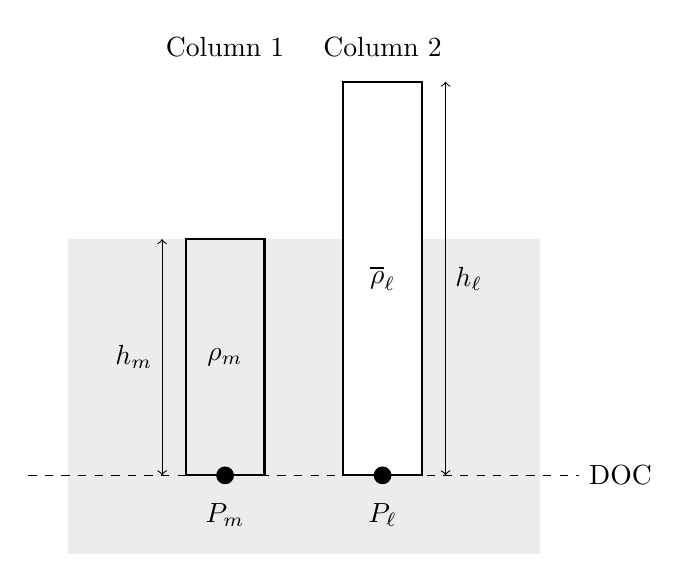
\begin{tikzpicture}[scale=1.0]

        % Asthenosphere
        \fill[gray!15] (-1.5,-1) rectangle (4.5,3);

        % Elevation difference
        \draw[<->] (-0.3,0) -- (-0.3,3) node[midway,left] {$h_m$};

        \draw[thick] (0,0) rectangle (1,3);
        \node[above] at (0.5,5.2) {Column 1};
        \draw[fill=black] (0.5,0) circle (3pt);
        \node at (0.5,1.5) {$\rho_m$};
        \node at (0.5,-0.5) {$P_m$};

        % Columns 1
        \draw[thick,fill=white] (2,0) rectangle (3,5);
        \node[above] at (2.5,5.2) {Column 2};
        \draw[fill=black] (2.5,0) circle (3pt);
        \node at (2.5,-0.5) {$P_\ell$};

        % Heights
        \draw[<->] (3.3,0) -- (3.3,5) node[midway,right] {$h_{\ell}$};

        % Compensation depth
        \draw[dashed] (-2,0) -- (5.0,0) node[right] {DOC};

        % Labels
        \node at (2.5,2.5) {$\overline{\rho}_{\ell}$};

    \end{tikzpicture}
    \caption{Schematic columns for the mantle and a column of lithosphere buoyantly supported at isostatic equilibrium. Pressure is balanced at a depth of compensation (DOC).}
    \label{fig:columns1}
\end{figure}

Isostatic equilibrium is therefore expressed as a balance of pressure at a common depth of equal normal stress.  Consider a vertical column of lithosphere of height $h_{\ell}$ and average density $\overline{\rho}_{\ell}$ overlying asthenospheric material of density $\rho_m$ (Figure~\ref{fig:columns1}).  The downward pressure exerted by the lithospheric column is
\[
    P_{\ell} = \overline{\rho}_{\ell} h_{\ell} g .
\]
For the column to be in isostatic equilibrium, this pressure must be balanced by the pressure of displaced asthenospheric material,
\[
    P_m = \rho_m h_m g ,
\]
where $h_m$ is the height of the displaced fluid column.  The net vertical pressure is given by
\[
    P_{\mathrm{net}} = 0 = \overline{\rho}_{\ell} h_{\ell} g - \rho_m h_m g .
\]

Importantly, this expression shows that isostasy depends on vertically integrated quantities.  Only the product of density \emph{and} thickness enters the balance; detailed vertical variations in density within the column are not resolved.  In this sense, isostasy provides no intrinsic vertical resolution.

\subsection{Lateral pressure balance and the depth of compensation}

Isostasy is fundamentally a lateral constraint.  Consider two neighboring lithospheric columns with different buoyancies and elevations (Figure~\ref{fig:columns2}).  For each column, the pressure balance may be written as
\begin{align*}
    \text{Column 1:} \quad 
    P_{\mathrm{net},1} &= \overline{\rho}_{\ell,1} h_{\ell,1} g - \rho_m h_{m,1} g , \\
    \text{Column 2:} \quad
    P_{\mathrm{net},2} &= \overline{\rho}_{\ell,2} h_{\ell,2} g - \rho_m h_{m,2} g .
\end{align*}
\begin{figure}[hbt]
    \centering
    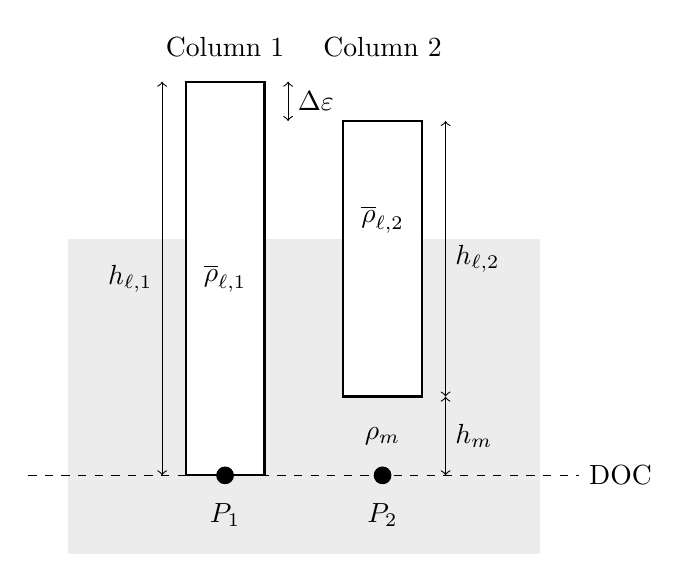
\begin{tikzpicture}[scale=1.0]

        % Asthenosphere
        \fill[gray!15] (-1.5,-1) rectangle (4.5,3);

        % Columns 1
        \draw[thick,fill=white] (0,0) rectangle (1,5);
        \node[above] at (0.5,5.2) {Column 1};
        \draw[fill=black] (0.5,0) circle (3pt);
        \node at (0.5,-0.5) {$P_1$};

        % Columns 2
        \draw[thick,fill=white] (2,1) rectangle (3,4.5);
        \node[above] at (2.5,5.2) {Column 2};
        \draw[fill=black] (2.5,0) circle (3pt);
        \node at (2.5,-0.5) {$P_2$};

        % Heights
        \draw[<->] (-0.3,0) -- (-0.3,5) node[midway,left] {$h_{\ell,1}$};
        \draw[<->] (3.3,0) -- (3.3,1) node[midway,right] {$h_m$};
        \draw[<->] (3.3,1) -- (3.3,4.5) node[midway,right] {$h_{\ell,2}$};
        \draw[<->] (1.3,4.5) -- (1.3,5) node[midway,right] {$\Delta\varepsilon$};

        % Compensation depth
        \draw[dashed] (-2,0) -- (5,0) node[right] {DOC};

        % Labels
        \node at (0.5,2.5) {$\overline{\rho}_{\ell,1}$};
        \node at (2.5,3.25) {$\overline{\rho}_{\ell,2}$};
        \node at (2.5,0.5) {$\rho_m$};

    \end{tikzpicture}
    \caption{Schematic lithospheric columns in isostatic equilibrium. Pressure is balanced at a common depth (DOC), while surface elevations differ due to variations in integrated buoyancy of each column.}
    \label{fig:columns2}
\end{figure}

If both columns are in isostatic equilibrium, their net pressures must be equal,
\begin{align*}
    P_{\mathrm{net},1} &= P_{\mathrm{net},2} , \\
    \overline{\rho}_{\ell,1} h_{\ell,1} g - \rho_m h_{m,1} g 
    &= \overline{\rho}_{\ell,2} h_{\ell,2} g - \rho_m h_{m,2} g .
\end{align*}

Rearranging gives
\begin{equation}
    \overline{\rho}_{\ell,1} h_{\ell,1} g
    =
    \overline{\rho}_{\ell,2} h_{\ell,2} g + \rho_m h_m g ,
    \label{eq:isostatic_pressure}
\end{equation}
where $h_m = h_{m,1} - h_{m,2}$.
Equation~\ref{eq:isostatic_pressure} expresses the requirement that pressures be equal at a common reference depth.
This depth is known as the \emph{depth (or level) of compensation} (Figure~\ref{fig:isostasy2}).

The equilibrium elevation difference between the two columns,
$\Delta \varepsilon = \varepsilon_1 - \varepsilon_2$,
may be written as
\begin{equation}
    \Delta \varepsilon = h_{\ell,1} - (h_{\ell,2} + h_m) .
    \label{eq:isostatic_elevation}
\end{equation}

Together, Eqs.~\ref{eq:isostatic_pressure} and \ref{eq:isostatic_elevation} show that differences in elevation arise from differences in column-integrated buoyancy.
Both density and thickness variations may contribute, and in general neither can be uniquely determined without additional assumptions.



\subsection{Interpretation and limitations}

In practice, lithospheric columns often consist of multiple layers.
In such cases the average density is an arithmetic weighted mean,
\begin{align*}
    \overline{\rho} &= \frac{1}{h} \sum_{i=1}^{N} \rho_i h_i , \\
    h &= \sum_{i=1}^{N} h_i .
\end{align*}

Isostatic analysis rests on several implicit assumptions:
\begin{itemize}
    \item Vertical forces other than buoyancy are negligible.
    Dynamic mantle flow may exert additional vertical stresses, producing elevation anomalies that are not isostatic in origin.
    \item The lithosphere offers no lateral resistance to deformation.
    In reality, lithospheric strength allows loads to be regionally supported by flexure; local isostasy is therefore best regarded as an end-member approximation.
    \item The system is in equilibrium.
    When density or thickness changes occur rapidly (e.g., glacial unloading, erosion, delamination), the lithosphere requires time to adjust toward a new isostatic state.
\end{itemize}

These limitations emphasize that isostasy is a constraint on admissible mass distributions, not a complete physical description of lithospheric deformation.
Gravity anomalies reflect both isostatic structure and departures from equilibrium, and isostasy therefore reduces—but does not eliminate—the non-uniqueness inherent in gravity interpretation.

\subsection{Local isostatic end-members}

\subsubsection{End-member nature of idealized models}

The simplest formulations of isostasy are local models, in which each lithospheric column is assumed to be independently supported by buoyancy forces.  Two classical end-member formulations, commonly known as Airy and Pratt isostasy, are widely used to illustrate how lateral variations in elevation may arise.

These models should be understood as \emph{limiting cases}, not as competing or mutually exclusive mechanisms.  Airy-type behavior isolates the effects of thickness variation at fixed density, whereas Pratt-type behavior isolates the effects of lateral density variation with a common base.  In the Earth, isostatic balance generally involves simultaneous variations in both density and thickness, and real solutions may be expressed as combinations of these end-members.

As a result, it is generally inappropriate to assign specific tectonic environments uniquely to one isostatic model.  The value of these end-members lies in their interpretive clarity rather than in their literal applicability.  Both end-members, and the general balance from which they derive, share the same underlying assumption of \emph{zero} lithospheric strength; Section~\ref{sec:regional_compensation} revisits this assumption directly.

\ntextbox{A brief history of local isostatic models}{

The two classical end-member models of local isostasy were published in the same year, 1855, but arose from very different motivations.  Archdeacon John Pratt developed his formulation while analyzing gravity observations collected across the Himalaya.  At that time, they didn't have gravimeters.  The direction of local vertical gravity was made by using a plumb line (a mass on the end of a spring) referenced to the stars for precise orientatation.  Pratt's measurements revealed an apparent mass deficiency beneath regions of high elevation, leading Pratt to propose that mountain ranges are underlain by lower density material rather than by thickened crust \citep{Pratt1855}.  In his interpretation, the base of the crust is flat, and surface topography reflects lateral variations in average density resulting from varying composition of the crust.

Later in the same year, Sir George Airy proposed an alternative explanation after reading Pratt's work \citep{Airy1855}.  Airy was the Astronomer Royal based at the Greenwich Royal Observatory at the time.  His office overlooked the Thames River.  In the spring, loggers would float felled trees down the river to the sawmills, providing inspiration for Airy's alternative model.  As an analogy for Earth's crust, Airy noted that all logs have similar density, those with larger diameters extend both higher above and deeper below the water surface.  This lead Airy to assume instead that crustal density is uniform and that surface relief is supported by variations in crustal thickness, with mountains underlain by buoyant roots extending into the mantle.

Although these formulations are often presented as competing models, neither is intended to describe all geological situations.  Rather, Pratt-type and Airy-type behavior represent limiting cases that isolate the roles of density and thickness variations, respectively.
Modern interpretations of isostasy generally involve combinations of both effects---lateral variations in both lithospheric density and thickness.
}{aside}

\subsubsection{Airy-type behavior}

In the Airy end-member, lithospheric density is assumed to be laterally uniform, while thickness varies.  Differences in surface elevation are accommodated by variations in the thickness of the crust, commonly conceptualized as buoyant roots extending into the underlying mantle.

Consider two crustal columns of equal density $\rho_c$, with one column thicker than the other (Figure~\ref{fig:isostasy}).  Let the thicker column extend to a deeper level through a compensating root beneath the region of higher elevation.  In this case, the difference in elevation $\Delta \varepsilon$ between the two columns may be written as
\[
    \Delta \varepsilon = (h_2 - h_1)\left(1 - \frac{\rho_c}{\rho_m}\right),
\]
where $\rho_m$ is the density of the underlying mantle.
\begin{figure}[hbt]
  \centering
  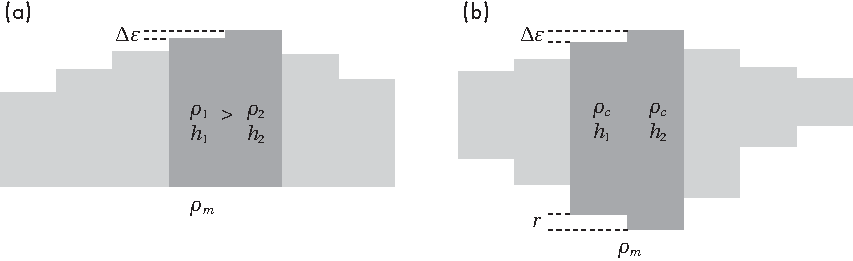
\includegraphics[]{gravity/figures/isostasy.pdf}
  \caption{Schematic comparison of (a) Pratt-type and (b) Airy-type local isostatic end-members. Both represent limiting cases of isostatic balance.}
  \label{fig:isostasy}
\end{figure}

Airy-type behavior is commonly invoked when interpreting crustal roots beneath mountain belts and plateaus.  However, isostatic balance alone does not uniquely constrain the geometry or depth extent of such roots.  Additional information from seismology or other geophysical observations is required to resolve vertical structure.

\subsubsection{Pratt-type behavior}

In the Pratt end-member, lithospheric thickness is assumed to be laterally uniform, while density varies from column to column.
Differences in elevation arise from lateral variations in mass per unit volume rather than from variations in thickness.

Historically, Pratt developed this formulation based on gravity observations across the Himalaya, which suggested a mass deficiency beneath regions of high elevation \citep{Pratt1855}.
In this interpretation, the base of the crust is flat, and topographic relief reflects decreasing average density toward the interior of the mountain range (Figure~\ref{fig:isostasy}a).
Airy later proposed the complementary thickness-variation model after reading Pratt's work \citep{Airy1855} (Figure~\ref{fig:isostasy}b).

For two crustal columns of equal thickness but different densities $\rho_1$ and $\rho_2$, the resulting elevation difference may be expressed as
\[
    \Delta \varepsilon = h \left(\frac{\rho_1}{\rho_2} - 1\right),
\]
where $h$ is the common column thickness.

Pratt-type behavior highlights the role of density variations arising from compositional differences or temperature variations.  For this reason, it provides a natural conceptual bridge to thermal isostasy, which is developed later in the chapter and revisited in the context of lithospheric cooling models (Chapter~\ref{ch:geothermics2}).

\section{Thermal Isostasy}\label{sec:thermal_isostasy}

Before connecting isostasy to gravity and flexure, it is useful to isolate the role of temperature.  Thermal isostasy arises from lateral variations in temperature that modify density and therefore buoyant support. In many tectonic settings, observed elevation differences cannot be explained solely by variations in crustal thickness or composition, but instead reflect differences in the thermal structure of the lithosphere and upper mantle.

A common strategy is to normalize each lithospheric column to a reference or \emph{standard column} defined by an average crustal thickness and average composition. Compositional and thickness effects are accounted for first, and any remaining elevation difference is then attributed to thermal buoyancy. In this framework, the total isostatic elevation difference may be written as
\begin{equation}
    \Delta \varepsilon_{\mathrm{total}}
    =
    \Delta \varepsilon_{\mathrm{compositional}}
    +
    \Delta \varepsilon_{\mathrm{thermal}} .
\end{equation}
This decomposition assumes local isostatic compensation and neglects flexure and dynamic pressure gradients in the mantle.

\subsection{Normalization to a standard column}

Consider a lithospheric column composed of \(N\) layers of thickness \(h_i\) and density \(\rho_i\), overlying a mantle of density \(\rho_m\). Let the reference column have corresponding quantities \(h_i^{\mathrm{ref}}\) and \(\rho_i^{\mathrm{ref}}\), chosen to represent average crustal structure.

Under local isostatic equilibrium, pressure balance at the depth of compensation requires that the vertically integrated mass of the column equal that of the reference column minus any elevation difference. The compositional and thickness contribution to elevation relative to the reference column is therefore
\begin{equation}
    \Delta \varepsilon_{\mathrm{compositional}}
    =
    \frac{1}{\rho_m}
    \sum_{i=1}^{N}
    \left(
        \rho_i h_i
        -
        \rho_i^{\mathrm{ref}} h_i^{\mathrm{ref}}
    \right).
\end{equation}

This expression corrects the observed elevation for differences in crustal thickness and composition relative to the standard column. Once this correction is applied, the remaining elevation signal is attributed to thermal effects.

\subsection{Thermal buoyancy and density variation}

Thermal isostasy follows from the temperature dependence of density. For small departures from a reference geotherm, density may be approximated as
\[
\rho(T) \approx \rho_0 \left[1 - \alpha \left(T - T_{\mathrm{ref}}\right)\right],
\]
where \(\alpha\) is the coefficient of thermal expansion, \(T(z)\) is the geotherm of interest, and \(T_{\mathrm{ref}}(z)\) is a reference geotherm.

Because isostasy depends on vertically integrated mass, the thermal contribution to elevation is obtained by integrating the temperature difference between the two columns,
\begin{equation}
    \Delta \varepsilon_{\mathrm{thermal}}
    =
    \alpha
    \int_{0}^{z_{\mathrm{max}}}
    \left[ T(z) - T_{\mathrm{ref}}(z) \right] \, dz,
\end{equation}
where \(z_{\mathrm{max}}\) is the depth over which thermal density differences contribute significantly to buoyancy.

\subsection{Piecewise geotherms}

In practice, geotherms are often represented as piecewise functions within depth intervals. In this case, the elevation contribution from the \(i\)-th depth interval is
\begin{equation}
    \varepsilon_i
    =
    \alpha
    \int_{z_i}^{z_{i+1}}
    \left[ T(z) - T_{\mathrm{ref}}(z) \right] \, dz,
\end{equation}
and the total thermal elevation is obtained by summing over all intervals,
\begin{equation}
    \Delta \varepsilon_{\mathrm{thermal}}
    =
    \sum_{i=1}^{N} \varepsilon_i .
\end{equation}

Because the integral operator is linear, each term may be evaluated by integrating the geotherms separately and taking the difference,
\begin{equation}
    \varepsilon_i
    =
    \alpha
    \left[
        \int_{z_i}^{z_{i+1}} T(z)\, dz
        -
        \int_{z_i}^{z_{i+1}} T_{\mathrm{ref}}(z)\, dz
    \right].
\end{equation}
This formulation makes no assumptions about the functional form of the geotherms.

Thermal isostasy provides a direct link between geothermics and surface observables. Cooling of the lithosphere increases density and produces subsidence, while elevated temperatures reduce density and produce buoyant uplift. These effects account for much of the long-wavelength elevation signal observed over oceanic plates, continental interiors, and magmatic provinces.

In later chapters, we return to thermal isostasy in the context of half-space and plate cooling models, where explicit geotherms are developed and time-dependent subsidence and uplift can be calculated. In those settings, thermal isostasy provides the physical connection between thermal evolution, surface topography, and long-wavelength gravity anomalies.


\section{Relationship between Gravity and Isostasy}

Gravity and isostasy are closely related but fundamentally distinct concepts.  Gravity describes the acceleration field produced by a distribution of mass, whereas isostasy describes a mechanical equilibrium state of that mass distribution.  As a result, gravity observations may reflect both isostatic equilibrium and departures from it, but gravity alone does not determine whether isostatic balance has been achieved.

In an isostatically compensated system, lateral variations in surface elevation are supported by corresponding variations in mass at depth.  These compensating masses reduce the long-wavelength gravity signal that would otherwise be produced by topography alone.  Conversely, gravity anomalies often arise from departures from perfect isostatic balance, whether due to incomplete compensation, lithospheric strength, or time-dependent adjustment.  In this sense, gravity anomalies provide information about isostatic state, not isostasy itself.

Isostasy therefore acts as a physically motivated constraint on gravity interpretation.  By restricting the class of admissible lateral mass distributions, isostatic assumptions reduce the non-uniqueness inherent in gravity analysis, but they do not eliminate it.  Different combinations of density and thickness variations can satisfy the same isostatic condition while producing similar gravity fields.

The connection between gravity and isostasy is most clearly seen by considering vertical force balance expressed as a pressure balance at a common depth of equal normal stress.  When written in terms of pressure, each contributing term is proportional to the product $\rho h g$.  Because the gravitational acceleration $g$ multiplies all terms equally, it cancels when pressures are equated between neighboring columns.  Isostatic equilibrium therefore does not depend on the magnitude of the gravity field, but on relative variations in vertically integrated mass.

This cancellation highlights an important conceptual point.  Isostasy is not a statement about the gravity field itself, but about buoyant support provided by the underlying mantle.  Gravity governs the weight of a column, but isostasy describes how that weight is balanced by the displacement of material at depth.  The absence of an explicit gravity term in the final equilibrium condition does not imply that gravity is irrelevant; rather, gravity has already been accounted for in establishing vertical force balance.

Because isostatic balance depends only on column-integrated quantities, it provides no direct information on how mass is distributed with depth within a column.  A shallow low-density anomaly and a deeper high-density anomaly may contribute equally to the pressure balance while producing very different gravity signatures.  This limitation underscores the complementary roles of gravity and isostasy: gravity is sensitive to the spatial distribution of mass, whereas isostasy constrains only the integrated effect required for mechanical equilibrium.

\subsection{Isostatic residual gravity}\label{sec:isostatic_residual}

Isostatic corrections are commonly applied to gravity data to suppress long-wavelength gravity variations associated with the isostatic support of topography. One widely used and operationally simple formulation is that of \citet{Simpson_etal1986}, who constructed an isostatic residual gravity map of the conterminous United States to emphasize gravity anomalies arising from lateral density variations within the crust.

\subsection{Conceptual basis}

The method of \citet{Simpson_etal1986} assumes local Airy--Heiskanen isostatic compensation. In this formulation, surface topography is supported by a crustal root of variable thickness and constant density contrast with the mantle. Because Bouguer and terrain corrections already remove the gravitational attraction of surface topography, the isostatic correction is applied to the Bouguer gravity anomaly and accounts only for the gravitational effect of the subsurface compensating mass.

The isostatic residual gravity anomaly is defined as
\[
    \Delta g_{\mathrm{iso\text{-}res}}(x,y) =
    \Delta g_{\mathrm{B}}(x,y) - \Delta g_{\mathrm{root}}(x,y),
\]
where $\Delta g_{\mathrm{B}}$ is the complete Bouguer anomaly and $\Delta g_{\mathrm{root}}$ is the gravity effect of the compensating crustal root.

Under local Airy isostasy, pressure balance at a common depth of compensation requires that the surface load be balanced by a buoyant root such that
\[
    \rho_c h(x,y) + \left( \rho_m - \rho_c \right) r(x,y) = 0,
\]
where $h(x,y)$ is the surface elevation relative to sea level, $\rho_c$ is the average crustal density, $\rho_m$ is the mantle density, and $r(x,y)$ is the thickness of the compensating root.

Solving for the root thickness yields
\[
    r(x,y)
    =
    \frac{\rho_c}{\rho_m - \rho_c}\, h(x,y).
\]
This relation allows the geometry of the compensating root to be determined directly from gridded topographic and bathymetric data.

The compensating root is treated as a subsurface density anomaly relative to the surrounding mantle with density contrast
\[
    \Delta \rho = \rho_c - \rho_m .
\]
For continental crust overlying denser mantle, this contrast is negative, and the root represents a mass deficit. The root extends downward from the Moho to the depth of compensation beneath regions of positive topography, and upward beneath regions of negative relief if bathymetry is included.

The gravity effect of the compensating root is computed using standard forward-gravity methods. In continuous form, the vertical component of the gravitational acceleration produced by the root at the observation point $\vb{r}$ is given by
\[
    \Delta g_{\mathrm{root}}(\vb{r}) =
    G \iiint
    \frac{\Delta \rho(\vb{r'}) \, (z - z')} {|\vb{r} - \vb{r'}|^3}
    \, \dd{V'} ,
\]
where the integral is taken over the volume occupied by the compensating root.

In practice, the root is discretized as a set of laterally varying vertical columns derived from gridded topography. The gravity effect is evaluated numerically and subtracted from the Bouguer anomaly to yield the isostatic residual gravity field \citep{Simpson_etal1986}.

\subsection{Interpretation of isostatic residual anomalies}

Isostatic residual gravity anomalies primarily reflect lateral density variations within the crust rather than the degree of isostatic compensation. Importantly, large residual anomalies can be produced by crustal heterogeneity even when the lithosphere is in complete local isostatic equilibrium.

Consequently, isostatic residual gravity maps are best interpreted as emphasizing the gravity signature of:
\begin{itemize}
    \item lateral density contrasts in the upper and middle crust,
    \item sedimentary basins and volcanic provinces,
    \item intrusive bodies and basement structure,
    \item regional tectonic fabrics.
\end{itemize}

\citet{Simpson_etal1986} emphasize that isostatic residual anomalies should not be interpreted as indicators of isostatic disequilibrium. Instead, the primary value of the correction is the suppression of long-wavelength gravity contributions associated with crustal thickness variations required to support topography.

\subsection{Relation to spectral filtering}

Although formulated in the spatial domain, the Simpson et~al.~(1986) isostatic correction effectively acts as a physically motivated long-wavelength gravity filter. Because isostatically compensated topography contributes mainly to long wavelengths, removing the gravity effect of the compensating root attenuates these wavelengths without imposing an arbitrary spectral cutoff.

This behavior explains why isostatic residual gravity maps often resemble high-pass filtered gravity fields, while retaining a clear physical interpretation tied to crustal buoyancy rather than purely mathematical filtering.

\subsection*{Summary}

Isostatic residual gravity anomalies are constructed by removing the gravity effect of an assumed compensating mass from the Bouguer gravity field. The method of \citet{Simpson_etal1986} provides a practical and widely adopted framework for isolating gravity signals associated with shallow crustal density variations, while explicitly acknowledging the interpretive limitations imposed by isostatic assumptions.

\section{Regional compensation and lithospheric strength}\label{sec:regional_compensation}

\subsection{Breakdown of local isostasy}
Local isostatic formulations assume that each lithospheric column responds independently to loading and unloading. Essentially, local isostasy assumes that the lithosphere holds no inherent strength. This assumption is reasonable at long wavelengths and over sufficiently long time scales, but it breaks down when loads vary over short horizontal distances or when the lithosphere possesses significant mechanical strength. In such cases, topographic and tectonic loads are supported not purely by buoyant forces, but in part by lithospheric flexure.

At short wavelengths, local Airy or Pratt isostasy predicts unrealistically large variations in crustal thickness or density. In reality, the lithosphere resists bending and shear, allowing loads to be distributed over a broader region. As a result, the degree of isostatic compensation decreases with decreasing wavelength. Loads that vary rapidly in space may be only partially compensated or even effectively uncompensated over geologic time scales.

This wavelength dependence of compensation is one of the clearest expressions of lithospheric strength and provides a natural transition from local isostasy to regional support mechanisms.

We will explore two types of models for regional compensation: partial support and flexural plate theory.  The partial support model is more of an approximation for flexural plates, but can simplify the analysis when the full rigor and complexity of flexural theory is not needed.

\subsection{Partial support of loads by lithospheric strength}

When the lithosphere has finite strength, it behaves as an elastic or viscoelastic plate overlying a weaker asthenosphere. Surface loads, such as mountain belts, volcanic edifices, ice sheets, or sedimentary basins, are then supported partly by buoyancy and partly by bending stresses within the lithosphere. This behavior is referred to as \emph{regional compensation}.

In the limiting case of infinite lithospheric strength, loads are fully supported elastically and no isostatic adjustment occurs. In the opposite limiting case of zero strength, local isostasy is recovered. Most tectonic settings lie between these extremes.

\subsection{Partial compensation models}

In many geological settings, observed loads are neither fully locally compensated nor fully uncompensated. Partial compensation models provide a simple and practical way to describe this intermediate behavior without explicitly modeling the underlying mechanical stresses.

The central concept is the \emph{degree of compensation}, commonly denoted by \(C\), where
\[
0 \le C \le 1.
\]
A value of \(C=1\) corresponds to complete local isostatic compensation, while \(C=0\) represents a fully uncompensated load supported entirely by lithospheric strength. Intermediate values indicate that only a fraction of the load is supported by buoyancy.

In its simplest form, partial compensation is implemented by scaling the compensating root predicted by local isostasy. For example, under an Airy formulation,
\[
r = C \, r_{\mathrm{Airy}},
\]
where \(r_{\mathrm{Airy}}\) is the root thickness predicted for full local compensation. The remaining fraction of the load is implicitly supported by elastic or flexural stresses in the lithosphere.

Partial compensation models are particularly useful in gravity interpretation. In the spectral domain, the observed gravity anomaly may be represented as a weighted combination of uncompensated and fully compensated responses,
\[
\hat{g}(k)
=
(1-C(k))\,\hat{g}_{\mathrm{topo}}(k)
+
C(k)\,\hat{g}_{\mathrm{Airy}}(k),
\]
where the compensation factor \(C(k)\) may vary with wavelength. This formulation provides a natural interpretive link to gravity--topography admittance and coherence analyzes, which estimate the effective degree of compensation directly from observations.

It is important to emphasize that partial compensation models are descriptive rather than predictive. They parameterize the outcome of load support but do not explain the physical mechanisms responsible for it. In practice, wavelength-dependent partial compensation arises naturally from lithospheric flexure: long-wavelength loads tend toward local compensation, while short-wavelength loads are increasingly supported elastically.

Viewed in this way, partial compensation models serve as a useful interpretive bridge between local isostasy and flexural theory, summarizing observable behavior without replacing the underlying physical description of lithospheric strength.

\subsection{Flexural plate theory}

Regional compensation is commonly described using thin elastic plate theory. In its simplest form, lithospheric flexure is governed by
\begin{equation}
D \nabla^4 w + (\rho_m - \rho_c) g w = q(x,y),
\end{equation}
where \( w(x,y) \) is the vertical deflection of the lithosphere, \( q(x,y) \) is the applied surface load, \( \rho_c \) and \( \rho_m \) are crustal and mantle densities respectively, and \( D \) is the flexural rigidity.

The second term represents the restorative buoyancy force associated with isostatic adjustment, while the fourth-order differential operator reflects the resistance of the lithosphere to bending. In this formulation, isostatic buoyancy acts as a distributed sink or source term that tends to restore equilibrium, but does not necessarily act locally beneath the applied load.

\subsection{Flexural rigidity and effective elastic thickness}

The flexural rigidity \( D \) is defined as
\begin{equation}
D = \frac{E T_e^3}{12(1-\nu^2)},
\end{equation}
where \( E \) is Young's modulus, \( \nu \) is Poisson's ratio, and \( T_e \) is the \emph{effective elastic thickness} of the lithosphere.

The effective elastic thickness is not a direct measure of physical plate thickness, but a parameter that captures the integrated mechanical behavior of the lithosphere over the time scale of loading. Higher values of \( T_e \) imply stronger lithosphere and greater regional support of loads, while lower values imply weaker lithosphere and more local isostatic response.

\subsection{Implications for gravity and isostatic interpretation}

Flexural support modifies both the geometry and the wavelength content of compensating masses at depth. Because regional compensation spreads mass over larger horizontal distances, the associated gravity anomalies have longer wavelengths and lower amplitudes than those predicted by local isostasy.

This behavior provides a qualitative link between gravity anomalies, load distribution, and lithospheric strength. Long-wavelength gravity anomalies may reflect regional or incomplete compensation rather than simple Airy root geometry, while short-wavelength gravity signals may indicate uncompensated or shallow density variations.

As a result, interpreting gravity data through the lens of isostasy requires careful consideration of lithospheric strength. Local isostatic corrections may overestimate compensation at short wavelengths, whereas flexural models provide a more realistic framework for understanding how the lithosphere supports loads over space and time.

\subsection{Worked examples of regional compensation}

The effects of lithospheric strength and regional compensation are most clearly illustrated through a small number of classic geological settings. In each case, surface or subsurface loading produces a flexural response that departs from local isostatic expectations and provides insight into lithospheric rigidity.

\subsubsection{Seamount loading of oceanic lithosphere}

Large volcanic seamounts impose substantial loads on the oceanic lithosphere. If local isostasy applied, the load would be supported directly beneath the edifice by a crustal root and limited flexure would occur. Instead, observations show broad-wavelength bathymetric deflection extending hundreds of kilometers from the load, indicating significant lithospheric strength.

In flexural terms, a seamount can be approximated as a surface load \( q(x,y) \) applied to an elastic plate. The resulting deflection satisfies
\begin{equation}
D \nabla^4 w + (\rho_m - \rho_w) g w = q(x,y),
\end{equation}
where \( \rho_w \) is seawater density. The characteristic decay length of deflection,
\[
\alpha = \left( \frac{4D}{(\rho_m - \rho_w) g} \right)^{1/4},
\]
controls the width of the flexural moat surrounding the seamount.

Bathymetric and gravity observations of seamount moats and peripheral bulges are commonly used to estimate the effective elastic thickness \(T_e\) of oceanic lithosphere. Younger lithosphere exhibits small \(T_e\) and narrow moats, while older lithosphere produces broader, lower-amplitude flexural responses, consistent with increasing lithospheric strength with age.

\subsection{Forward flexural solutions and estimation of elastic thickness}

Rather than treating all loads as locally compensated, lithospheric flexure provides a forward model that predicts surface deflection as a function of lithospheric rigidity. Observed surface topography and gravity signals can then be used to invert for the effective elastic thickness, \(T_e\). Two canonical end-member geometries are subduction zone bending and normal fault loading.

\subsubsection{Subduction zone bending and the outer rise}

The approach to a subduction trench subjects the incoming oceanic plate to bending moments that produce downward deflection at the trench and an upward flexural bulge seaward of it, known as the outer rise. The lithosphere may be approximated as an elastic plate overlying a buoyant asthenosphere.

For one-dimensional flexure perpendicular to the trench axis, the governing equation in the absence of distributed loading away from the trench is
\begin{equation}
D \frac{d^4 w}{dx^4} + (\rho_m - \rho_w) g w = 0,
\end{equation}
where \(w(x)\) is vertical deflection, \(\rho_m\) is mantle density, and \(\rho_w\) is seawater density.

The general solution that decays away from the trench is
\begin{equation}
w(x) = w_0 \, e^{-x/\alpha}
\left[
\cos\!\left(\frac{x}{\alpha}\right)
+
\sin\!\left(\frac{x}{\alpha}\right)
\right],
\end{equation}
where the flexural parameter
\begin{equation}
\alpha = \left( \frac{4D}{(\rho_m - \rho_w) g} \right)^{1/4}
\label{eq:flexural_parameter}
\end{equation}
controls both the wavelength and decay of the response.

This forward solution predicts:
\begin{itemize}
  \item a negative deflection at the trench,
  \item a positive deflection (outer rise) seaward of the trench,
  \item a characteristic wavelength proportional to \( \alpha \).
\end{itemize}

The position of the outer-rise crest occurs at approximately
\begin{equation}
x_{\mathrm{crest}} \approx \frac{\pi}{4}\,\alpha.
\end{equation}
Observed outer-rise wavelength therefore provides a direct constraint on \( \alpha \), and hence on \( D \) and \(T_e\).

\subsubsection{Normal fault loading and footwall uplift}

Large normal faults impose distributed loads on the lithosphere through hanging-wall subsidence and basin infilling. The resulting unloading of the footwall generates flexural uplift that extends well beyond the fault trace.

Assuming the fault at \(x=0\), we model the hanging wall as a uniform surface load of magnitude \(q_0\) applied over \(x>0\). The governing equation is
\begin{equation}
D \frac{d^4 w}{dx^4} + (\rho_m - \rho_c) g w = q(x),
\end{equation}
where
\[
q(x) =
\begin{cases}
q_0, & x > 0, \\
0, & x < 0.
\end{cases}
\]

The forward solution for deflection on the footwall side (\(x<0\)) is
\begin{equation}
w(x) = A \, e^{x/\alpha} \cos\!\left(\frac{x}{\alpha}\right),
\end{equation}
where the flexural parameter is now
\begin{equation}
\alpha = \left( \frac{4D}{(\rho_m - \rho_c) g} \right)^{1/4}.
\end{equation}

This solution predicts:
\begin{itemize}
  \item maximum uplift at a finite distance from the fault,
  \item uplift wavelength controlled by \( \alpha \),
  \item asymmetric topography across the fault.
\end{itemize}

Observed footwall uplift width and amplitude may therefore be used to estimate \( \alpha \), constraining \(T_e\) through the flexural rigidity.

\subsubsection{Inversion for effective elastic thickness}

In both geometries, observations of surface deflection constrain \( \alpha \). Once \( \alpha \) is estimated, the flexural rigidity follows from Eq.~\eqref{eq:flexural_parameter}, and the effective elastic thickness is obtained from
\begin{equation}
D = \frac{E T_e^3}{12(1-\nu^2)},
\end{equation}
where \(E\) is Young's modulus and \(\nu\) is Poisson's ratio.

These forward models highlight the central role of lithospheric strength in controlling regional compensation. Where local isostasy predicts narrow, column-scale responses, flexural theory predicts broad, wavelength-dependent deformation whose geometry directly encodes information about lithospheric rheology.

\section{Flexural equilibrium topography and gravity anomalies}

Flexural models predict the surface deflection of the lithosphere in response to applied loads. These deflections are accompanied by mass redistribution both at the surface and at depth, which together generate a gravity anomaly. Relating flexural topography to gravity provides the final link between lithospheric strength, regional compensation, and observed gravity fields.

\subsection{Mass contributions associated with flexure}

A flexural deflection \(w(x,y)\) produces two primary contributions to the gravity field:

\begin{enumerate}
    \item A surface topographic mass associated with the deflection of the surface.
    \item A subsurface buoyancy anomaly associated with displacement of material at the base of the plate.
\end{enumerate}

For simplicity, consider a lithosphere of density \(\rho_c\) overlying mantle of density \(\rho_m\). A downward deflection corresponds to thickening of the crust and replacement of lighter material by denser mantle material at depth.

\subsection{Gravity effect of surface deflection}

Under the Bouguer slab approximation, the gravity anomaly associated with surface deflection is
\begin{equation}
\Delta g_{\mathrm{surf}}(x,y) = 2\pi G \rho_c \, w(x,y),
\end{equation}
where \(w\) is positive upward.

This term represents the gravitational attraction of the surface load and is removed by the Bouguer correction when working with Bouguer gravity anomalies.

\subsection{Gravity effect of flexural compensation}

Flexural deflection also produces a subsurface mass anomaly due to displacement of the crust--mantle boundary. If the Moho is assumed to follow the flexural deflection with reduced amplitude, the gravity contribution of this deep interface is
\begin{equation}
\Delta g_{\mathrm{root}}(x,y)
=
2\pi G (\rho_c - \rho_m)\, w(x,y)\, e^{-|\mathbf{k}|T_0}
\quad \text{(Fourier domain)} ,
\end{equation}
where \(T_0\) is the mean depth to the compensating interface and the exponential term accounts for attenuation of short wavelengths with depth.

This expression highlights a crucial difference between local isostasy and flexure: under flexural support, subsurface mass redistribution is spread laterally and attenuated at short wavelengths.

\subsection{Net gravity anomaly from flexural support}

The total gravity anomaly associated with flexural deformation is the sum of surface and subsurface contributions:
\begin{equation}
\Delta g(\mathbf{k})
=
2\pi G \rho_c \hat{w}(\mathbf{k})
\left[
1 -
\frac{\rho_m - \rho_c}{\rho_c}
e^{-|\mathbf{k}|T_0}
\right].
\end{equation}

If the Bouguer correction has already removed the surface contribution, the remaining gravity signal reflects only the subsurface flexural compensation.

At long wavelengths (\(|\mathbf{k}| \to 0\)), the compensation term approaches the Airy isostatic limit. At short wavelengths, the exponential term suppresses subsurface contributions, and surface loads dominate.

\subsection{Wavelength dependence and lithospheric strength}

Because flexural deflection depends on the flexural parameter
\[
\alpha = \left( \frac{4D}{(\rho_m - \rho_c) g} \right)^{1/4},
\]
the resulting gravity anomaly inherits the same wavelength dependence.

Strong lithosphere (large \(T_e\)) produces:
\begin{itemize}
    \item broad flexural wavelengths,
    \item regional subsurface mass redistribution,
    \item long-wavelength gravity anomalies.
\end{itemize}

Weak lithosphere (small \(T_e\)) produces:
\begin{itemize}
    \item short-wavelength deformation,
    \item near-local compensation,
    \item gravity anomalies resembling Airy isostasy.
\end{itemize}

\subsection{Connection to gravity admittance}

In the Fourier domain, the ratio of gravity to topography,
\begin{equation}
Z(|\mathbf{k}|) = \frac{\hat{g}(|\mathbf{k}|)}{\hat{w}(|\mathbf{k}|)},
\end{equation}
is known as the gravity admittance.

For a flexural plate, \(Z(|\mathbf{k}|)\) decreases with decreasing wavelength, reflecting the diminishing role of subsurface compensation at short wavelengths. Observed admittance curves therefore provide a powerful means of estimating elastic thickness and distinguishing between local and regional compensation.

\subsection{Interpretive implications}

Flexural equilibrium topography and its associated gravity anomaly form a coupled system. Topography encodes lithospheric strength through its wavelength and amplitude, while gravity encodes how mass is redistributed to support that topography.

This relationship emphasizes that gravity anomalies over tectonic loads are not solely indicators of density variations, but also reflect the mechanical behavior of the lithosphere. Interpreting gravity in tectonic settings therefore requires explicit consideration of flexural support and regional compensation.

\subsubsection{Key lessons from the examples}

These examples illustrate several important principles:
\begin{itemize}
    \item Short-wavelength loads are increasingly supported by lithospheric strength rather than local buoyancy.
    \item Flexural wavelengths and gravity anomalies provide direct constraints on effective elastic thickness.
    \item Regional compensation spreads mass laterally, producing long-wavelength gravity signals distinct from those predicted by local isostasy.
\end{itemize}

Taken together, the preceding examples illustrate several general principles governing how the lithosphere supports loads and how those loads are expressed in topography and gravity.

First, the assumption of local isostatic compensation becomes increasingly inappropriate at short wavelengths. As the horizontal scale of a load decreases, lithospheric strength allows stresses to be transmitted laterally, reducing the degree of local buoyant support. In these cases, surface loads are supported in part by elastic bending rather than by a compensating mass directly beneath the load.

Second, the characteristic wavelength of flexural deformation provides a direct constraint on lithospheric rigidity. Observed patterns of topography, bathymetry, and associated gravity anomalies encode information about the flexural parameter and therefore about the effective elastic thickness. These observations allow lithospheric strength to be estimated through forward and inverse modeling of flexural response.

Third, regional compensation spreads mass laterally over distances much larger than the load itself. This redistribution of mass produces gravity anomalies with longer wavelengths and lower amplitudes than those predicted by local isostatic models. As a result, long-wavelength gravity signals commonly reflect lithospheric strength and flexural support rather than simple variations in crustal thickness.

Together, these cases demonstrate that lithospheric flexure is not a special or exceptional circumstance, but a fundamental control on the mechanical response of the Earth to loads. Isostasy defines an equilibrium state, but the manner in which that state is approached—and the gravity signals that result—are strongly governed by lithospheric strength and the spatial scale of loading.

Together, these cases demonstrate that lithospheric flexure is not a special circumstance but a fundamental control on how the Earth supports loads across a wide range of tectonic environments.


\section{Isostatic disequilibrium and restorative processes}

Isostasy describes a state of mechanical equilibrium, but the Earth is rarely observed in that state instantaneously. Instead, the lithosphere and mantle are commonly observed to be in various stages of adjustment toward or away from isostatic balance. Distinguishing between isostatic equilibrium and the dynamic approach toward equilibrium is therefore essential for interpreting gravity, topography, and deformation.

\subsection{Equilibrium versus adjustment}

Isostatic equilibrium refers to the condition in which vertical stresses are balanced at a common compensation depth. By contrast, isostatic disequilibrium reflects a transient state in which mass distributions have changed more rapidly than the lithosphere and mantle can respond.

Such departures may arise from a variety of processes, including surface loading and unloading (e.g., volcanism, erosion, sedimentation, glaciation), tectonic thinning or thickening of the lithosphere, and thermal evolution of the mantle. When these processes operate on time scales short compared with the viscous relaxation time of the mantle or the viscoelastic response time of the lithosphere, isostatic balance is temporarily violated.

\subsection{Time dependence of the isostatic response}

Isostatic adjustment is not instantaneous because the mantle behaves as a highly viscous solid. Although pressure gradients generated by mass redistribution provide a restoring buoyancy force, the rate at which the system responds is controlled by mantle viscosity and lithospheric strength.

As a result, isostatic response is inherently time dependent. Loads emplaced rapidly may be partly supported by elastic stresses or flexural bending, with buoyant adjustment occurring gradually through viscous flow. Over sufficiently long time scales, elastic stresses relax and the system approaches a new equilibrium state.

This temporal distinction parallels the contrast between steady-state heat flow and transient thermal diffusion developed in later chapters: equilibrium solutions describe end states, while the path toward those states depends on material properties and process rates.

\ntextbox{Timescale of Rebound}{
    A useful conceptual model for glacial isostatic adjustment treats rebound as the time-dependent relaxation of a buoyant load through a highly viscous mantle. The goal of this model is not to predict detailed uplift histories, but to establish how characteristic time scales arise from mantle viscosity and load wavelength.

    Consider a load of characteristic horizontal scale \(\lambda\) (e.g., an ice sheet) that is applied rapidly and later removed. The lithosphere responds elastically, while the underlying mantle behaves as a linear viscous medium with viscosity \(\eta\). Following unloading, buoyancy provides a restoring force that drives vertical motion toward a new isostatic equilibrium.

    In this simplified framework, the vertical displacement \(w(t)\) at a representative point evolves as
    \begin{equation}
    w(t) = w_\infty \left(1 - e^{-t/\tau}\right),
    \end{equation}
    where \(w_\infty\) is the final equilibrium uplift and \(\tau\) is the characteristic rebound time.

    Dimensional analysis shows that the rebound time scale depends on mantle viscosity, buoyancy, and load wavelength,
    \begin{equation}
    \tau \sim \frac{\eta}{\Delta \rho\, g\, \lambda},
    \end{equation}
    where \(\Delta\rho\) is the density contrast driving buoyant restoration and \(g\) is gravitational acceleration. Long-wavelength loads therefore relax more slowly than short-wavelength loads, and higher mantle viscosity leads to longer rebound times.

    This simple relation captures several key observations of glacial isostatic adjustment:
    \begin{itemize}
        \item uplift continues long after ice sheets have retreated,
        \item rebound rates depend on the horizontal scale of loading,
        \item observed vertical velocities provide direct constraints on mantle viscosity.
    \end{itemize}

    Although real GIA involves elastic lithosphere, layered mantle viscosity, and additional feedbacks, this single-timescale model encapsulates the essential physics of restorative buoyancy acting through a viscous mantle. In this sense, glacial isostatic adjustment provides a clear illustration of isostasy as a state, and rebound as the time-dependent process by which that state is approached.

    \paragraph{Order-of-magnitude estimate for the Baltic Ice Sheet.}

    As a simple example, consider the postglacial rebound of the Baltic Shield following removal of the Baltic Ice Sheet. A reasonable characteristic wavelength for the load is
    \[
    \lambda \sim 1000~\mathrm{km},
    \]
    corresponding to the lateral extent of major uplift patterns in Fennoscandia.

    The dominant buoyancy contrast driving rebound is between mantle material and surface water/air, which we approximate as
    \[
    \Delta\rho \sim 2300~\mathrm{kg\,m^{-3}}.
    \]
    Adopting a representative mantle viscosity beneath the Baltic Shield of
    \[
    \eta \sim 10^{21}~\mathrm{Pa\,s},
    \]
    the characteristic rebound time scale is
    \begin{align}
    \tau 
    &\sim \frac{10^{21}}{(2300)(9.8)(1\times10^{6})} \\
    &\sim 4\times10^{10}~\mathrm{s} \\
    &\sim 1.3\times10^{3}~\mathrm{yr}.
    \end{align}

    This estimate lies within an order of magnitude of uplift time scales inferred from geodetic and geological observations, especially when considering that longer effective wavelengths and slightly higher viscosities would increase the predicted time constant to several thousand years.

    This simple calculation illustrates why glacial isostatic rebound persists long after ice retreat and why observed uplift rates in Fennoscandia provide direct constraints on mantle viscosity. Although real GIA involves elastic lithosphere, layered viscosity, and additional feedbacks, this single-timescale model captures the essential physics of restorative buoyancy acting through a viscous mantle. In this sense, glacial isostatic adjustment provides a clear illustration of isostasy as a state, and rebound as the time-dependent process by which that state is approached.
}{core}

\subsection{Gravity and topography as indicators of disequilibrium}

Departures from isostatic balance are expressed in both gravity and topography. Uncompensated or partially compensated loads produce gravity anomalies whose amplitude and wavelength differ from those expected under local isostatic assumptions. Similarly, topography that is higher or lower than predicted by isostatic models may indicate incomplete adjustment or additional supporting mechanisms.

In the spectral domain, gravity--topography coherence provides a powerful diagnostic of compensation. High coherence at long wavelengths and reduced coherence at short wavelengths are consistent with regional compensation and lithospheric strength, whereas low coherence at long wavelengths may signal disequilibrium or dynamic support from mantle flow. Such analyzes quantify the degree of compensation as a function of wavelength, rather than assuming a fixed isostatic model.

\subsection{Observing contemporary isostatic adjustment}

In some settings, isostatic adjustment is occurring rapidly enough to be observed directly. Geodetic measurements of vertical velocities reveal ongoing uplift or subsidence associated with processes such as postglacial rebound, sediment loading, volcanic inflation, and tectonic exhumation.

These observations provide direct constraints on the rate of isostatic response and, when combined with gravity and topography, allow inferences about mantle viscosity and lithospheric rheology. Contemporary vertical motions thus complement static gravity observations by adding a temporal dimension to the interpretation of isostatic processes.

\subsection{Linking flexure, viscous flow, and gravity}

The mechanical response of the Earth to loading reflects the combined effects of elastic flexure in the lithosphere and viscous flow in the mantle. Flexure governs the immediate spatial pattern of deformation and partial support of loads, while mantle viscosity controls the rate at which buoyant equilibrium is restored.

Gravity anomalies integrate these effects. Short-wavelength anomalies often reflect elastic or flexural support, whereas long-wavelength gravity signals are sensitive to regional compensation and viscous relaxation. Interpreting gravity data therefore requires consideration of both mechanical state and temporal evolution.

Viewed in this context, isostatic disequilibrium is not an exception to isostatic theory, but an expected consequence of the Earth's finite strength and viscosity. Gravity, topography, and geodetic observations together provide complementary constraints on how rapidly and over what spatial scales the Earth responds to perturbations in mass distribution.

\section{Summary}
\begin{itemize}
  \item Isostasy constrains permissible lateral mass distributions but does not uniquely define structure.
  \item Gravity reflects both equilibrium and disequilibrium components of mass distribution.
  \item Departures from isostatic equilibrium provide insight into lithospheric strength, mantle rheology, and ongoing geodynamic processes.
  \item Thermal, compositional, and mechanical effects together determine the observed isostatic state of the Earth.
\end{itemize}

Isostasy defines a mechanically admissible equilibrium state for lateral mass distributions, but it does not specify how that state is achieved or how long it takes.  Glacial isostatic adjustment, post-orogenic collapse, and the subsidence of cooling oceanic plates all illustrate systems evolving toward isostatic balance through different physical processes.  Gravity, topography, and geodetic observations together allow us to distinguish equilibrium structure from ongoing adjustment.  This distinction between state and process will reappear, particularly in the context of steady-state geotherms (Chapter~\ref{ch:geotherics1}) and time-dependent thermal diffusion (Chapter~\ref{ch:geothermics2}).

When doing an isostatic analysis, we typically assume that the columns are in equilibrium resulting from buoyancy forces only.  As a result of this assumption, there are several implict requirements for this to be true:
\begin{itemize}
    \item Additional vertical pressures contributed from dynamic processes are negligible; otherwise, forces in addition to buoyancy will result in an elevation anomaly.  As an example, upward flow in mantle convection can exert a vertical pressure (force per given area) on the lithospheric column and reduce the pressure applied from buoyancy resulting in a postive elevation anomaly.  Likewise, downward flow from subduction can relate in negative elevation anomalies.

    \item The lithosphere has zero lateral strength; otherwise, the lithosphere could flex, violating isostatic equilibrium.  There are two things working on our side here.  First, over long geologic times and/or high lithospheric temperatures, the lithosphere is relatively weak allowing it to adjust to near equilibrium.  Second, if we take a large enough region (larger than the flexural wavelength of the lithosphere) we can also assume that the departures from equilibrium are small.

    \item The forces acting on the column are in equilibrium; otherwise, its elevation will adjust to some level different than where it currently lies.  When a column's density and/or height change (e.g., metamorphism, glacial retreat, evaporation of a large lake, mantle delamination), the column must adjust to a new elevation.  If these processes occur fast enough, the lithosphere will take time to adjust.
\end{itemize}

Viewed together, local isostasy, thermal buoyancy, flexural support, partial compensation, and time-dependent adjustment represent different limits of a unified framework linking mass, temperature, strength, topography, and gravity across space and time.


\nocite{Watts2001}

\bibliographystyle{elsarticle-harv}
\bibliography{ref}